\documentclass[10pt]{article}
\usepackage[margin=1in]{geometry}
\usepackage{titlesec}
\usepackage{graphicx}
\usepackage{amsmath}

% Title formatting
\titleformat{\section}{\large\bfseries}{\thesection}{1em}{}
\titleformat{\subsection}{\normalsize\bfseries}{\thesubsection}{1em}{}

\newcommand{\irow}[1]{% inline row vector
  \begin{smallmatrix}[#1]\end{smallmatrix}%
}

\begin{document}

\begin{center}
    {\LARGE \textbf{Accelerating BFS algorithms on FPGA}} \\[10pt]
    \textbf{Ethan Gabizon (ehg54), Tomas Choi (tic3), Dylan Lee (dl634)}
\end{center}

\section{Introduction}
\noindent We implement an optimized breadth first search algorithm on FPGA. Traditional graph algorithms 
are difficult to implement efficiently on a general-purpose CPU because of their irregular memory 
access patterns. They also tend to be memory-intensive rather than compute-intensive because they 
involve traversals, in which values get read and then almost immediately written back to memory with 
very little compute in between. We use the Alveo U280 card and leverage its high-bandwidth memory to 
accelerate BFS. First, we modify the representation of the BFS problem by using the coordinate format (COO).
Then, we implement a BFS traversal over a graph as a series of sparse-matrix-dense-vector multiplies; this 
approach of implementing graph algorithms with linear algebra is known as GraphBLAS. We optimize this BFS 
by instantiating multiple processing elements that can concurrently perform SPMV on different rows. To 
benchmark our designs, we use graphs from the SuiteSparse Matrix Collection. We compare our optimized designs
against the unoptimized FPGA design.

\section{Background}
\subsection{Alveo U280 FPGA Platform}
\noindent For the labs, we use the Zedboard, but for this final project we use the Alveo U280 card. The Alveo U280 
card is a data center accelerator card containing a more powerful FPGA due to its capacity, bandwidth, and 
power efficiency. Figure~\ref{fig:u250} shows the Alveo block diagram for the U250 card (it is still relevant for 
the description of the U280 card). The FPGA is divided into two partitions, shell and user. The shell partition 
is a static region that provides the basic control and communication for things like PCIe connectivity, board 
management, clocking, and reset. The user partition is a dynamic region that contains the user compiled binary,
so the hardware that we synthesize. There is a PCIe interface for the host and FPGA to communicate with each
other. The PCIe interface will allow the transfer of data between the host and the device memory, where the device 
memory could be PLRAM, HBM, or DDR. \newline

\begin{figure}[h!]
  \centering
  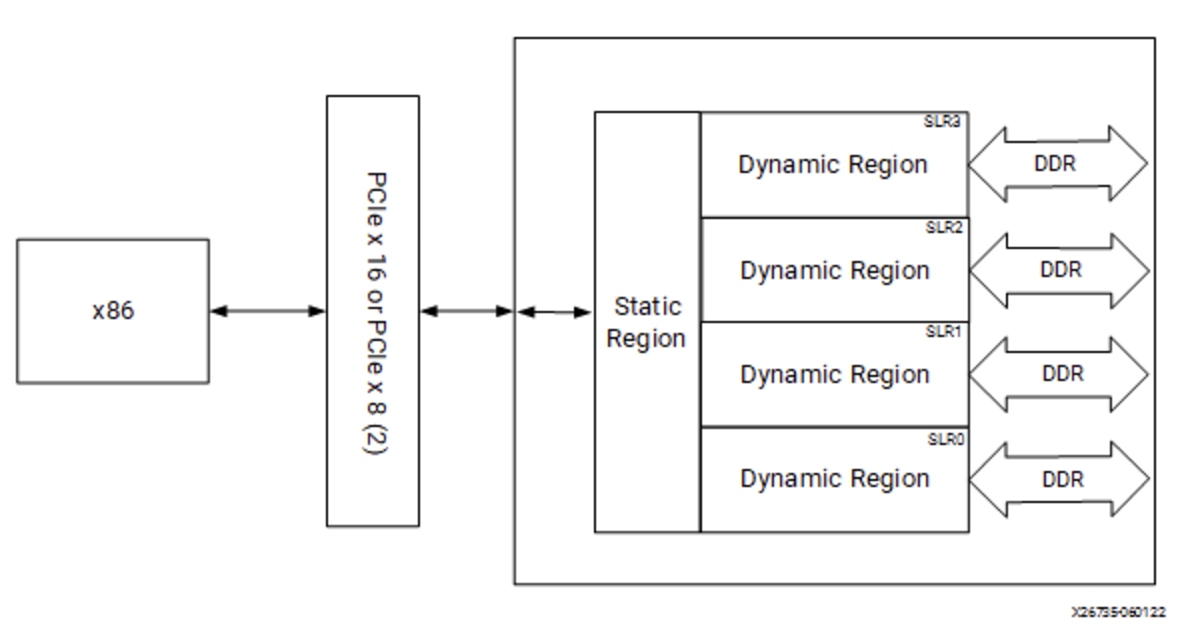
\includegraphics[width=0.5\textwidth]{u250.png}
  \caption{U250 Block Diagram}
  \label{fig:u250}
\end{figure}

\noindent For our project, we only used HBM. High bandwidth memory is a high performance memory technology that 
allows for massive memory bandwidth by exposing multiple memory channels to the processing units. Figure~\ref{fig:hbm} 
shows the HBM subsystem in the U280 card. It contains two HBM stacks, and each has 16 pseudo channels. Above the pseudo 
channels, there are 16 memory channels that each control two pseudo channels. Then, there is a switch network for 
every two memory channels that exposes 4 AXI interfaces, so in total there are 32 AXI ports. For our project, we 
use a maximum of 18 of these because our designs range from using one HBM channel to 16 just for coordinate data. 
It is important to emphasize that HBM allows our memory bound workload of BFS to be pushed computationally. 

\begin{figure}[h!]
  \centering
  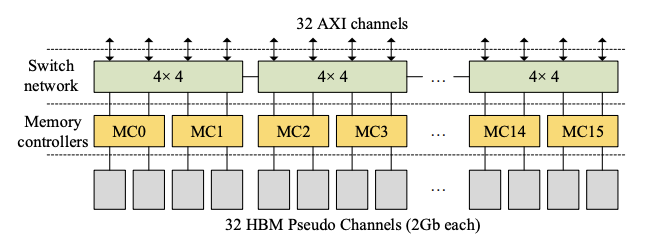
\includegraphics[width=0.5\textwidth]{hbm.png}
  \caption{HBM Subsystem in U280 Card}
  \label{fig:hbm}
\end{figure}

\subsection{HLS Directives}
\noindent To optimize our design, we use multiple HLS directives: dataflow, interface, loop tripcount,
array partition, pipeline, and unroll. For this report, we focus on the ones that most students 
in ECE6775 are not familiar with. First, the \textbf{dataflow} pragma enables task-level parallelism. 
This allows functions and loops to overlap in their operation. If there are any consumer and producer 
relationships in the dataflow region, then their respective functions will need to wait for each 
other. If there are none, then all of the functions could run concurrently. The Vitis HLS tool 
will try to minimize the overall latency and improve concurrency by starting operations as soon 
as data is available. Second, the \textbf{interface} pragma specifies how RTL ports are created from 
the function definition during interface synthesis. This pragma defines how data is passed between 
the design and the external world. It determines the communication protocol, data handling, and 
optimization of memory access for ports, arrays, and variables in the design. Lastly, the 
\textbf{loop tripcount} directive is used to specify the minimum, maximum, and average trips that a 
loop might take. This directive is only used for analysis and it does not actually affect the synthesis 
results. We used it to specify the trip count of our variable bound loops to have better estimates of 
latency while optimizing our design.

\section{Problem Description}

\subsection{BFS}
\noindent We begin by giving a high level overview of BFS. Breadth First Search is a graph traversal algorithm
in which you start at a node and traverse all of its adjacent nodes. Once all the adjacent nodes are visited,
then those nodes' adjacent nodes are visited. Figure~\ref{fig:bfs_graph} shows an example traversal order. 
The common opposite to Breadth First Search is Depth First Search where you start at a node, traverse to an 
adjacent node, and traverse all nodes reachable through that adjacent node before moving on to the next adjacent
node. \newline

\begin{figure}[h!]
  \centering
  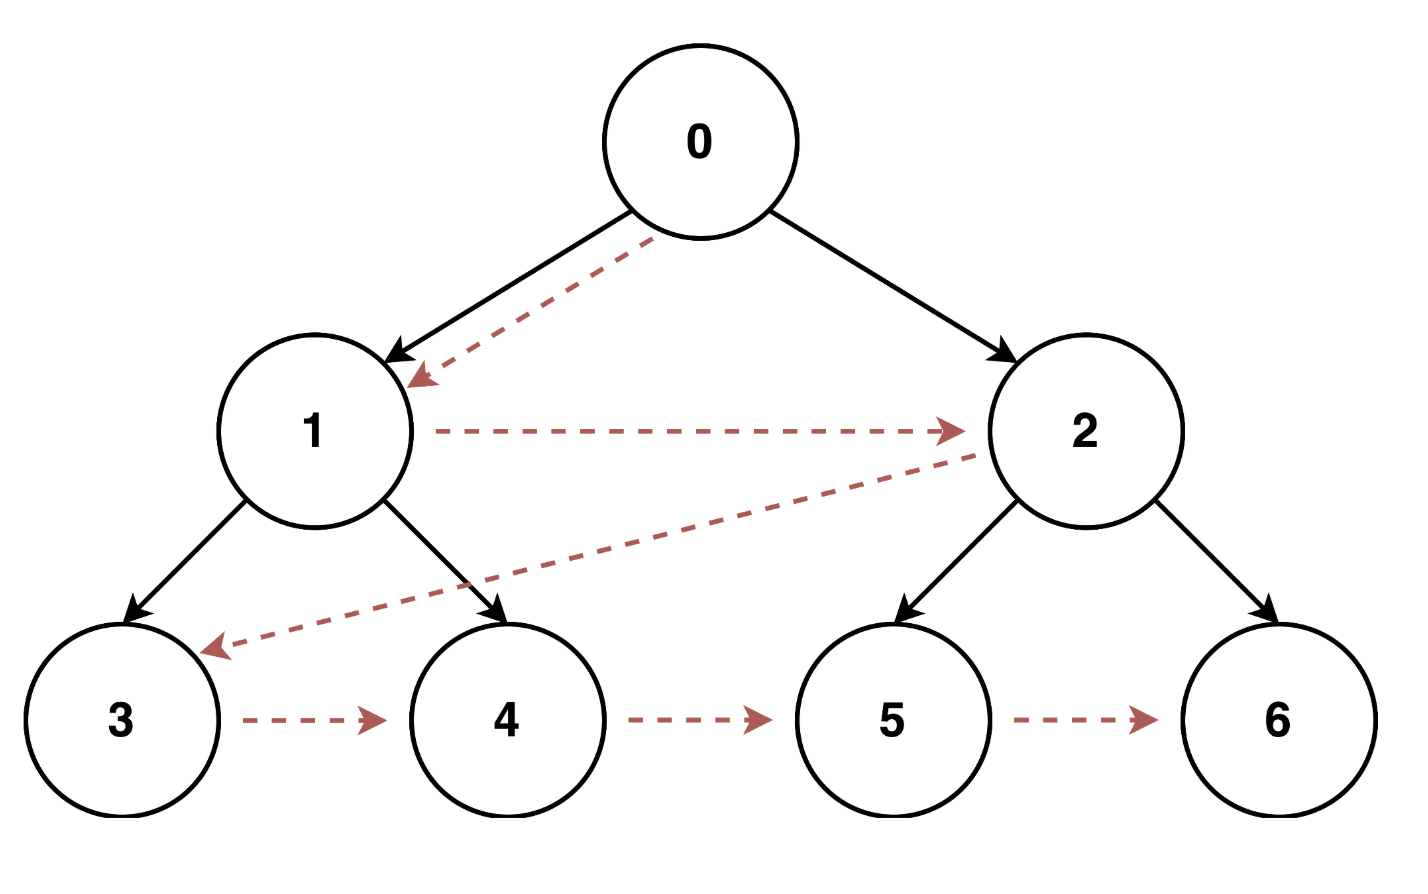
\includegraphics[width=0.5\textwidth]{bfs_graph.png}
  \caption{BFS Example Traversal Order}
  \label{fig:bfs_graph}
\end{figure}

\subsection{BFS with Linear Algebra}
\noindent Instead of the traditional way to implement graph algorithms, we take advantage of the fact that a graph can 
be represented as a matrix to which linear transformations can be applied to perform these graph operations.
We use sparse matrix multiplication to perform our BFS algorithm. This is a common way to perform BFS as documented
in the GraphBLAS specification. We can represent graphs using adjacency matrices in which the value at (i, j) in the 
matrix represents the presence of an edge and possibly a weight between nodes i and j. In our case, these weights will
be 0 or 1 to simply represent the presence of an edge. Using these matrices, we can perform BFS by iteratively conducting 
matrix vector multiplication with the adjacency matrix and a vector that represents the frontier, where a 1 in the ith 
in the frontier means that node i will be explored. Figure~\ref{fig:adj_matrix} shows the way in which the example in 
Figure~\ref{fig:bfs_graph} is mapped to an adjacency matrix that facilitates matrix vector operations.

\begin{figure}[h!]
  \centering
  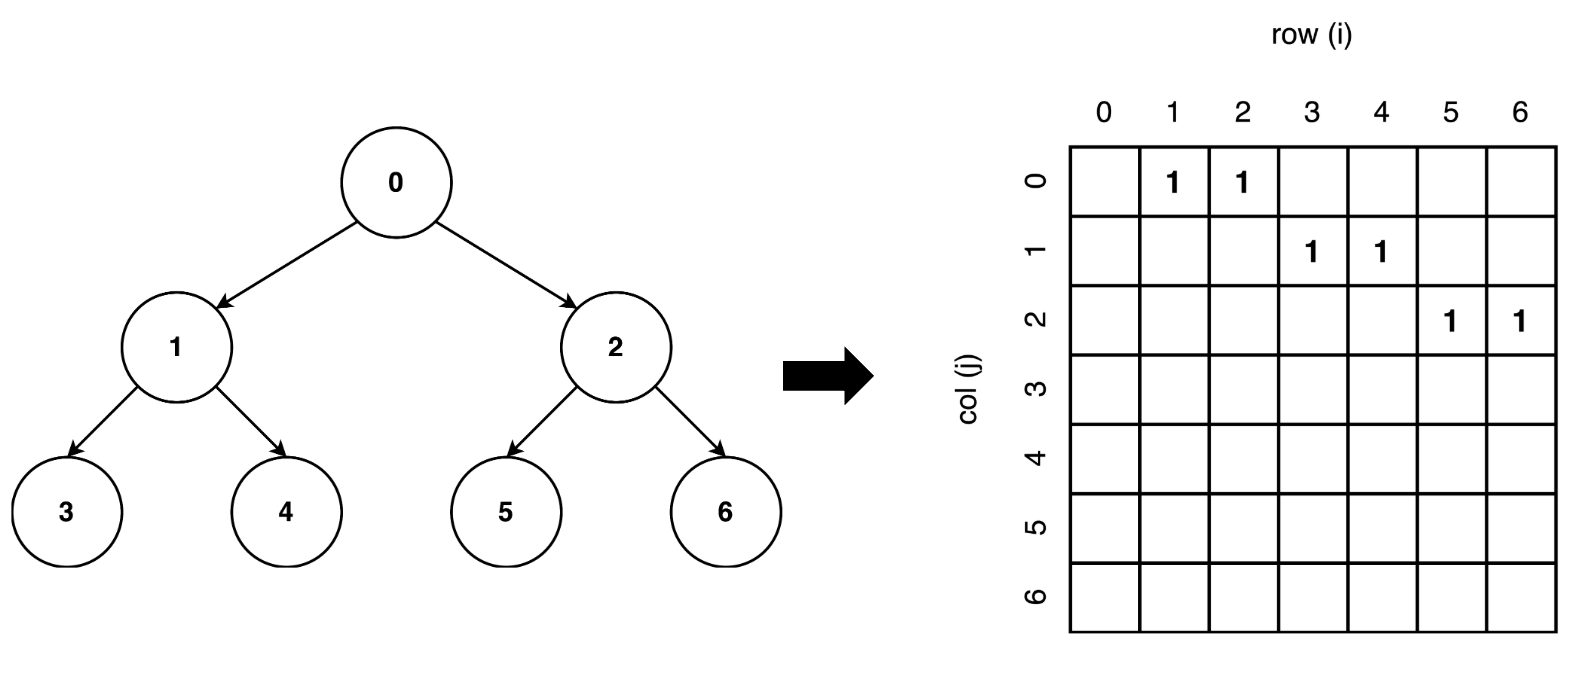
\includegraphics[width=0.5\textwidth]{adj_matrix.png}
  \caption{Adjacency Matrix Representation of Graph}
  \label{fig:adj_matrix}
\end{figure}

\subsection{Architecture}

\noindent Our application takes as input a matrix encoded as a graph, using the COO
format. For our benchmarks, we use matrices from the Suite Sparse Matrix
Collection. While this data is not particularly meaningful as a graph (the
matrices often represent data important to algorithms in various domains), they
provided us with access to many sparse matrices so we did not have to generate
our own. Also, the Suite Sparse matrices are already encoded in COO format,
eliminating one step of pre-processing we would need to do. \newline

\noindent Our application also takes an integer, $hops$, which specifies how many levels
from the start node in the graph to traverse. Our algorithm outputs the frontier
of nodes at that level, $frontier$. For example, using the graph in
Figure~\ref{fig:adj_matrix}, with $hops=1$, the output would be $frontier =
\irow{0 & 1 & 1 & 0 & 0 & 0 & 0}$ because nodes 1 and 2 are 1 hop away from the
start node. Similarly, with $hops=2$, the output would be $frontier=\irow{0 & 0
& 0 & 1 & 1 & 1 & 1}$. \newline

\noindent The steps to our baseline application are shown in
Figure~\ref{fig:baseline_impl}. The host code is responsible for reading the
matrix from the specified file, and parses it into a COO vector (with the row
and column indices packed into a single 32-bit integer) that our application
takes as input. It also specifies the number of hops. Then, it sends that data
to the FPGA, which initializes the memories it uses to store intermediate
results and then performs an iterative algorithm of repeated SpMVs. After each
SpMV, our kernel updates the current visited set of nodes based on the output of
that iteration's SpMV. Logically, if a node was not already visited and not in
the frontier set returned by the SpMV, it remains unvisited. If it was
previously visited, it stays visited. If it was not already visited and is in
the frontier set, we mark it as visited. Using the updated visited set, we apply
a mask to the SpMV output to ensure that we only visit a node once. After this
step, if there are more hops to make (meaning more iterations), we jump back to
doing the SpMV. If not, we write the most recent SpMV result to our kernel
output, which we then transfer back to the host. \newline

\begin{figure}[h!]
  \centering
  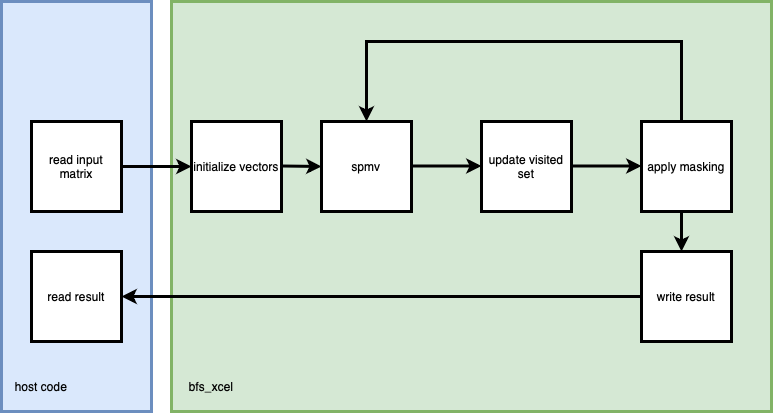
\includegraphics[width=0.75\textwidth]{bfs_unopt.png}
  \caption{Baseline Implementation}
  \label{fig:baseline_impl}
\end{figure}

\noindent This is our baseline design, but we identify that the SpMV kernel is a major
source of parallelism. Most of the application is memory-bound, meaning it is
bottlenecked by the amount of data we can access from memory at any given time
rather than the number of computations we can do. SpMV, however, is simply a
series of accumulating logical ORs; so, to speed up our application we first
looked to optimize SpMV by dividing the work among several PEs. We discuss these
optimizations in the next section, as well as the implications it has for our
application's memory hierarchy.

\section{Implementation}

\subsection{Base Design}
\noindent Our baseline implementation, which targets the U280 FPGA, is represented in
Figure~\ref{fig:baseline_impl}. Specifically, we make use of the board's high-bandwidth memory, shown in
Figure~\ref{fig:hbm} and Figure~\ref{fig:u250}, to transfer the matrix from the host to the FPGA.

\subsection{8 PE Design}
\noindent We identified that one of the bottlenecks of our base design was how fast we could compute each SpMV.
In order to accelerate it, we split the computation up into 8 processing elements, which would each 
handle the computations for a smaller part of the matrix, and we would have additional hardware
to merge their results. The design of the SpMV kernel is shown in Figure~\ref{fig:spmv_diagram} and the
design of each PE is shown in Figure~\ref{fig:pe_diagram}. As a heuristic for load balancing, we also
assign rows to each PE cyclically. For example, PE 0 works on rows 0, 8, 16, and so on, while PE 1 works
on 1, 9, 17, and so on. These sets of COO values are split into 8 HBM channels, one for each PE. \newline

\begin{figure}[h!]
  \centering
  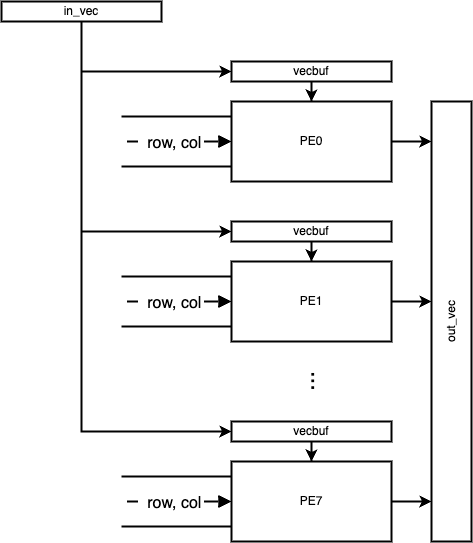
\includegraphics[width=0.5\textwidth]{spmv_diagram.png}
  \caption{Parallelized SpMV}
  \label{fig:spmv_diagram}
\end{figure}

\begin{figure}[h!]
  \centering
  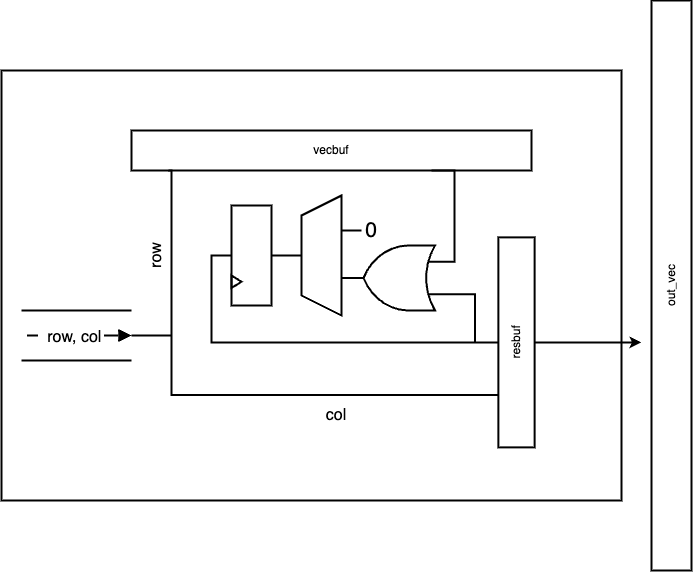
\includegraphics[width=0.5\textwidth]{pe_diagram.png}
  \caption{SpMV Processing Element}
  \label{fig:pe_diagram}
\end{figure}

\noindent In order to apply the dataflow pragma to our SpMV kernel, each PE had to read and write to its own
memories that the others did not touch. This means that we had to broadcast the BFS \verb|in_vec| argument
to 8 separate arrays, one for each PE. In Figure~\ref{fig:spmv_diagram}, this is represented by the
arrows pointing from the block labeled \verb|in_vec| to all the blocks titled \verb|vecbuf|. Additionally,
this implementation also requires us to partition the matrix into 8 blocks, one for each PE, in the host
code. We do this by modifying the interface to the BFS kernel. Now, it must take 8 arrays which represent
the rows and columns that each PE must process. It also requires us to sort the matrix entires by row;
this is done in the host code as well. The matrix data that each PE uses is represented as an HLS stream,
or a FIFO. Each PE reads data from its own stream when it is ready to process it. \newline

\noindent Additionally, each PE writes to its own output vector. We slightly modify our BFS algorithm to work
on this data format, as the baseline only has 1 PE, so there is only one output vector. The logic remains
the same, however, and we merge these 8 separate output vectors into a single vector after all of the
SpMV iterations have completed. This output vector is then communicated back to the host device. A diagram
of the modified, optimized version that uses PEs is shown in Figure~\ref{fig:bfs_opt}. \newline

\begin{figure}[h!]
  \centering
  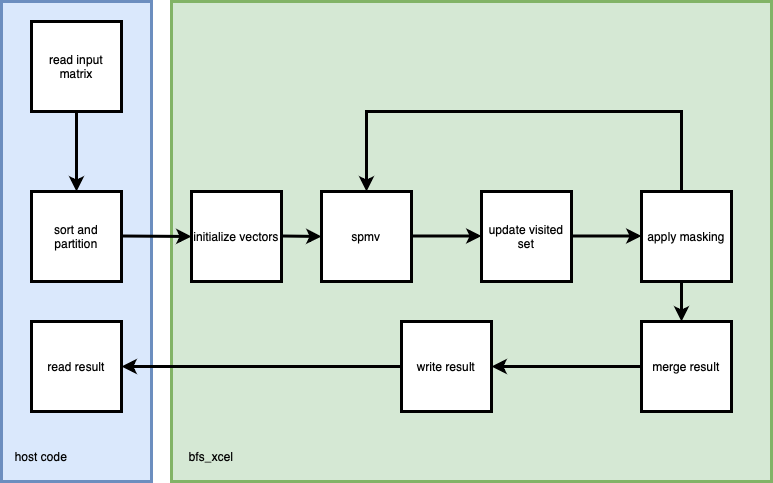
\includegraphics[width=0.75\textwidth]{bfs_opt.png}
  \caption{Optimized Implementation}
  \label{fig:bfs_opt}
\end{figure}

\noindent One concern with this implementation is the added overhead required to set up
our data to be processed by 8 PEs in parallel. Specifically, the additional
computations we had to perform are sorting the matrix by row, splitting it into
8 different blocks for each PE, broadcasting the input vector to each PE, and
combining the output vectors. The first two are done in the host code and take
the longest. A more detailed breakdown of total execution time by section is
shown in the evaluation section, but here we make the analysis that we can
amortize the pre-processing of the matrix across over many searches over that
graph. In many applications of a BFS algorithm, it is likely that multiple
searches may be performed over the same graph, so we feel that this is a fair
analysis. As such, we only compare the FPGA execution time of the BFS itself
across our baseline and optimized designs. Still, this adds the overhead of
broadcasting the input vectors and combining the output vectors. To mitigate the
effects of these operations on the total runtime, we applied optimizations to
unroll and pipeline the loops that broadcast the input vectors. We also modified our algorithm,
as stated previously, to only combine each PE's output vector at the end of the entire BFS instead
of after each SpMV (which is what we did initially). By reducing the number of times we need to merge
vectors, we were able to cut down on the overhead incurred by having multiple PEs. As a whole, we 
were able to achieve a speedup, which is discussed further in the evaluation.

\subsection{16 PE Design}
\noindent We also wrote a design that uses 16 PEs with 16 HBM channels, which has an overall structure
identical to the 8 PE design with 8 HBM channels. However, we found that this design actually does
not achieve a speedup over our baseline. We will discuss further in our
evaluation, but our hypothesis is that are dataset does not contain matrices
with a large enough number of nonzero entries to warrant that many PEs. As a
result, the overhead of having so many PEs (broadcasting inputs, merging
outputs) outweighs the performance boost we might get from computing more of
each SpMV in parallel, compared to having only 8 PEs.

\section{Testing}
\noindent We tested our designs and optimizations iteratively. At the beginning of our project timeline, we 
wrote our SpMV and BFS kernels and ran them in software to verify their correctness. Because we did not
have a trusted baseline to compare to for correctness, we generated several random matrices and 
ran our BFS algorithm by hand to ensure that the software implementation was correct. Once we verified
it this way for small examples, we trusted that it was correct because the logic was also quite simple. \newline

\noindent Next, using the software implementation as our source of truth, we implemented the host code to orchestrate
data movement between the CPU and the FPGA running our BFS algorithm. This way, we could implement our designs
in hardware, run them on the FPGA, and compare the results to the software implementation. When we made
major changes, like trying various optimizations, our first step was to run software emulation and ensure
that the optimizations maintained the correct functionality of our kernel. \newline 

\noindent We also verified all of our designs this way with hardware emulation and bitstream generation. We wanted
to ensure that there was no unexpected behavior when applying optimizations or compiling the design
to hardware. There were instances where hardware emulation caught bugs arising from the incorrect use
of certain optimization pragmas, which weren't apparent in software emulation. As a whole, this end-to-end
testing strategy made us confident that our optimized designs were also correct.

\section{Evaluation}
% \textit{Students should describe the experimental setup used to evaluate their design. Students
% should describe the data inputs used to evaluate their design and provide an analysis of the achieved
% results. The results should be clearly summarized in terms of tables, text, and/or plots. Please provide
% qualitative and quantitative analysis of the results and discuss insights from these results. Results may
% include (but are not limited to) the execution time of an algorithm, hardware resource usage, achievable
% throughput, and error rate. It would be interesting, for example, to discuss why one design is better
% than another, why one design achieves a higher metric than another, or how you trade-off one metric
% for another. Consider going into detail for one particular instance of your experiment and analyze how
% it achieves the given results}

\noindent We evaluated our designs across a series of 7 benchmarks, each of which have a number of nonzero entries ranging
from several hundred to 4096, since 4096 is the largest number of nonzero entries our implementation can handle. 

\begin{figure}[h!]
  \centering
  \begin{tabular} {| c | c | c | c | c | c | c | c |}
    \hline
                    & young\_4c & 685\_bus & 1138\_bus & ash292 & lp\_nug06 & lund\_b & olm1000 \\
    \hline
    base            & 10.485    & 10.405   & 10.410    & 10.393 & 10.414    & 10.4002 & 10.430 \\
    \hline
    8 PE            & 4.853     & 7.204    & 6.467     & 8.022  & 6.964     & 7.989   & 5.153 \\
    \hline
    8 PE Processing & 7.861     & 8.820    & 9.060     & 8.475  & 8.995     & 8.601   & 8.958 \\
    \hline
    16 PE           & 5.466     & 7.277    & 6.549     & 8.1532 & 6.943     & 8.090   & 5.905 \\
    \hline
    16 PE Processing& 7.959     & 10.675   &   11.1232 & 9.298  & 9.847     & 9.783   & 8.703 \\
    \hline
  \end{tabular}
  \caption{Execution Time Breakdown, in ms}
  \label{fig:exec_times}
\end{figure}

\begin{figure}[h!]
  \centering
  \begin{tabular} {| c | c | c | c | c | c | c | c |}
    \hline
         & young\_4c & 685\_bus & 1138\_bus & ash292 & lp\_nug06 & lund\_b & olm1000 \\
    \hline
    N    & 841       & 685      & 1138      & 292    & 486       & 147     & 1000 \\
    \hline
    NNZ  & 4089      & 1967     &  2596     & 1250   & 2232      & 1294    & 3996 \\
    \hline
  \end{tabular}
  \caption{Benchmark characteristics}
  \label{fig:bench_info}
\end{figure}

\begin{figure}[h!]
  \centering
  
\includegraphics[width=0.75\textwidth]{speedup.png}
  \caption{Preprocessing times and speedup over base}
  \label{fig:speedups}
\end{figure}

\begin{figure}[h!]
  \centering
  \begin{tabular} {| c | c | c | c | c | c | c |}
    \hline
          & BRAM \% & FF \% & LUT \% & BRAM SLR \% & FF SLR \% & LUT SLR \% \\
    \hline
    base  & 0 & 0 & 2 & 0 & 0 & 0 \\
    \hline
    8 PE  & 0 & 2 & 10 & 0 & 0 & 3 \\
    \hline
    16 PE & 0 & 8 & 53 & 0 & 2 & 17 \\
    \hline
  \end{tabular}
  \caption{Resource usage}
  \label{fig:resources}
\end{figure}

\noindent Figure~\ref{fig:exec_times} displays the execution time of each of our designs, separating out the FPGA execution time from
the host preprocessing time. Figure~\ref{fig:bench_info} contains the characteristics of each benchmark, where N is the number of
rows and columns in the matrix and NNZ is the number of nonzero entries. Since these are sparse matrices, it is true for all the
benchmarks that $\mathit{NNZ} << N^2$. Figure ~\ref{fig:speedups} shows the preprocessing times and the respective speedup that the 8 and 
16 PE designs achieve over the baseline design. Figure ~\ref{fig:resources} shows the resource usage across our different designs.\newline

\noindent We observe several trends. First, we note that the 16 PE design never outperforms the 8 PE design. However, the 16 PE design
uses many more resources than the 8 PE design, particularly LUTs. The disparity in resource usage can likely be attributed to
the extra data storage and the associated logic for accessing/routing it, which is needed as the number of PEs grows. We hypothesize
that the 16 PE design underperforms the 8 PE design because the overhead required to coordinate data movement between the PEs is far
greater than the amount of parallelism we gain in computing each SpMV. As we discussed previously, introducing parallel PEs requires
additional time to broadcast each SpMV input vector, as well as merge the output vector at the end of the BFS. Furthermore, our
design operates on relatively small matrices. We hypothesize that the 8 PE design already achieves much of the parallelism that is
possible from the computation of each SpMV, and the rest of the time is dominated by data movement. As a result, there is not
much parallelism for the 16 PE design to take advantage of. However, we predict that if we were to evaluate benchmarks with more
nonzero entries, the 16 PE design would probably achieve speedups greater than the 8 PE design.\newline

\noindent We also note that the speedup is greatest on the young\_4c and olm1000 benchmarks. We hypothesize that this is due to these
benchmarks achieving the best load balancing. Both of these benchmarks have nonzero entries closest to our limit, 4096. This
means that each PE is doing an almost equal amount of work, whereas in other benchmarks some PEs are likely doing more work
than others. As a result, the load balanced benchmarks achieve a greater speedup because they take advantage of more parallelism
than the ones that are not load balanced.

\section{Project Management}

\noindent Throughout the 6 weeks of our project, we met every 2-3 days to catch up on the work we have done and to set up
milestones for the next time we meet. This ensured that everyone had something to do and made the project
progress little by little. The steps to the completion of our project are generalized as 1) get familiar with
Vitis framework and new FPGA, 2) implement SpMV and BFS accelerators, and 3) optimize accelerators. Everything went
smoothly with a minor inconvenience of the server update, which required us to change our workflow a little bit. \newline

\noindent \textbf{Week 1 (11/05 - 11/12)}:
\begin{itemize}
  \item Set up Vitis framework on example vvadd kernel with all hardware targets (Tomas)
  \item Set up flow to read SuiteSparseMatrix dataset (Ethan)
  \item Implement software SpMV on COO (Dylan)
\end{itemize}

\noindent \textbf{Week 2 (11/12 - 11/19)}:
\begin{itemize}
  \item Test software implementation of SpMV with COO format (Dylan)
  \item Write SpMV kernel and test bench for traditional HLS flow, verify with random tests (Ethan)
  \item Set up Vitis framework on SpMV kernel with all hardware targets (Tomas, Dylan)
  \item Implement BFS implementation that uses the SPMV kernel (Tomas, Ethan)
  \item Create random testbench for BFS (Ethan)
  \item Set up Vitis framework for BFS (Tomas)
\end{itemize}

\noindent \textbf{Week 3 (11/19 - 11/26)}:
\begin{itemize}
  \item Concatenate row and data value of COO coordinate into one int value (Tomas)
  \item Optimize spmv kernel by instantiating multiple PEs, coordinating data movement between them, and apply dataflow optimizations (Ethan)
  \item Attempt to synthesize BFS for small sizes (Ethan)
  \item Create diagrams for SpMV and BFS (Dylan)
\end{itemize}

\noindent \textbf{Week 4 (11/26 - 12/03)}:
\begin{itemize}
  \item Refactor code to run unoptimized kernel, for a baseline comparison (Ethan)
  \item Write code to run kernels with Vivado tool, for debugging (Ethan)
  \item Fix code to handle dataflow pragma correctly (Tomas)
  \item Refactor BFS code to include the number of hops to make, instead of full traversal (Ethan)
  \item Incorporate SuiteSparseMatrix into code (Tomas, Dylan)
\end{itemize}

\noindent \textbf{Week 5 (12/03 - 12/10)}:
\begin{itemize}
  \item Set up timing framework: preprocessing vs. FPGA (Ethan)
  \item Write BFS implementation with 16 PEs (Tomas)
  \item Synthesize baseline, 8 PE, 16 PE implementations (Dylan)
  \item Profile implementations to determine small speedup (Ethan)
  \item Unroll some loops related to buffering of input and output (Ethan)
  \item Optimize code by eliminating need of output buffer merging (Tomas)
\end{itemize}

\noindent \textbf{Week 6 (12/10 - 12/17)}:
\begin{itemize}
  \item Record presentation (Dylan, Ethan, Tomas)
  \item Write report (Dylan, Ethan, Tomas)
\end{itemize}

\section{Conclusion}

\noindent In this project, we explore the acceleration of BFS by exploiting linear algebra 
operations, high-bandwidth memory, and data level parallelism. By representing graphs in
COO format, we are able to perform sparse matrix vector multiplication on the represented graph
to perform fast traversals. To minimize the memory bound nature of BFS, we use the HBM 
channels in the U280 FPGA platform to concurrently read different row data from device memory.
Lastly, we take advantage of the fact that the SpMV operations can be performed concurrently for 
different rows to distribute the workload into different processing elements. We investigate
for designs with a single PE with one HBM channel, 8 PEs with 8 HBM channels, and 16 PEs with 16 HBM
channels and observe speedups from the 8 PE design due to data level parallelism but 
less speedup from the 16 PE design due to communication overhead. Throughout the course of the 
project, we have learned about the Vitis software, the U280 card, GraphBLAS concepts, new HLS directives
like dataflow and interface, and testing and profiling techniques to evaluate our designs. We would
like to acknowledge the significant help we received from Yixiao to get set up for the bigger FPGA, 
to learn about GraphBLAS, and to debug significant problems. 

\end{document}